%\documentclass[]{beamer}
\documentclass[handout]{beamer}
%\documentclass[handout,draft]{beamer}

% Preambulo
% Paquetes para usar bien el idioma español
\usepackage[spanish,es-tabla]{babel}
\selectlanguage{spanish}
\usepackage[utf8]{inputenc}

% Paquetes para usar mejores imagenes
\usepackage{graphicx}

% Paquetes para links y tabla de contenidos en el PDF
\usepackage{hyperref}
\hypersetup{colorlinks=true,allcolors=blue}
%\usepackage{hypcap}

% Paquetes para mejores tablas
\usepackage{booktabs}

% Mejor matematica
\usepackage{amsmath}

% Fuentes de las imagenes
\usepackage[absolute,overlay]{textpos}

% Paquete captions
\usepackage[justification=centering,labelformat=empty,labelsep=none]{caption}

% Opciones para ticks
\usepackage{tikz}
\usetikzlibrary{shapes,arrows,positioning}

\tikzstyle{decision} = [diamond, draw, fill=blue!20, text width=4em, text badly centered, node distance=2cm, inner sep=0pt,on grid]
\tikzstyle{block} = [rectangle, draw, fill=blue!20, text width=8em, text centered, rounded corners, minimum height=2em,on grid]
\tikzstyle{line} = [draw, -latex]

% Citas bibliograficas
\usepackage[backend=biber]{biblatex}
\renewcommand{\footnotesize}{\tiny}
\addbibresource{biblio.bib}

% Mejoro las captions
\setbeamertemplate{caption}{\raggedright\insertcaption\par}

\setbeamertemplate{caption}{%
\begin{beamercolorbox}[wd=0.85\paperwidth, sep=.2ex]{block body}\insertcaption%
\end{beamercolorbox}%
}


% Sacar barra de navegacion
\setbeamertemplate{navigation symbols}{}%remove navigation symbols

% Transparencias en items
\setbeamercovered{transparent}

% Estilo de diapositivas
% \usetheme{Boadilla}
\usecolortheme{whale}
\usecolortheme{orchid}


\title{Herramientas de Teledetección Cuantitativa\\{\small Clase 3}}
\author{Francisco Nemi\~na}
\institute{Unidad de Educaci\'on y Formaci\'on Masiva \\ Comisi\'on Nacional de
Actividades Espaciales}
%\institute[Inst.]{
\includegraphics[height=1cm]{Figures/logosopi.png}\phantom{pepe} 
\includegraphics[height=1cm]{Figures/2mp.png}\phantom{pepe} 
\includegraphics[height=1cm]{Figures/conae.png}}
\date{}
%\titlegraphic{
%\includegraphics[height=1cm]{IMAGENES/minplan.png}\phantom{1}
%
\includegraphics[height=1cm]{IMAGENES/conae.png}\phantom{1}
%
\includegraphics[height=1cm]{IMAGENES/sopi.png}}

\logo{
\includegraphics[height=0.7cm]{imagenes/sopi.png}}

\AtBeginSection[]
{\begin{frame}
\frametitle{Esquema de presentaci\'on}
\tableofcontents[currentsection]
\end{frame}
}


\begin{document}
\begin{frame}
    \maketitle
\end{frame}

\section{Transformaciones}
\subsection{Motivaci\'on}

\begin{frame}{Motivaci\'on}
  \begin{center}
      \resizebox{0.4 \linewidth}{!}{%
        \begin{tikzpicture}[node distance = 2cm, auto]
          \node[block]                                (init) {Firma Espectral};\pause
          \node[block, below= of init]                (resp) {Reflectancia Espectral Efectiva};
          \path[line] (init) --          (resp);
          \pause
          \node[decision, below= of resp]             (ques) {????};
          \path[line] (resp) --          (ques);\pause
        \end{tikzpicture}%
      }%
    \end{center}
\end{frame}
%--- Next Frame ---%

\begin{frame}{Motivaci\'on}
  \begin{block}{T\'ecnicas de reducci\'on de la dimensionalidad}
    \begin{itemize}[<+>]
      \item \'Indices
      \item Rotaciones
      \item Clasificaciones
    \end{itemize}
    \pause
    Empecemos con la primera.
  \end{block}
\end{frame}
%--- Next Frame ---%

\section{\'Indices}

\begin{frame}{\'Indices}
  \begin{block}{\'Indices}
    \begin{itemize}[<+>]
      \item Nos van a permitir reducir mas la dimensi\'onalidad.
      \item Perdiendo informaci\'on.
      \item Ganando y mucho en la interpretaci\'on de los resultados.
      \item Adem\'as voy a encontrar correlaciones con variables biof\'isicas.
    \end{itemize}
  \end{block}
\end{frame}
%--- Next Frame ---%

\subsection{\'Indices de Vegetaci\'on}

\begin{frame}{\'Indices de Vegetaci\'on}
    \begin{figure}
    \centering
    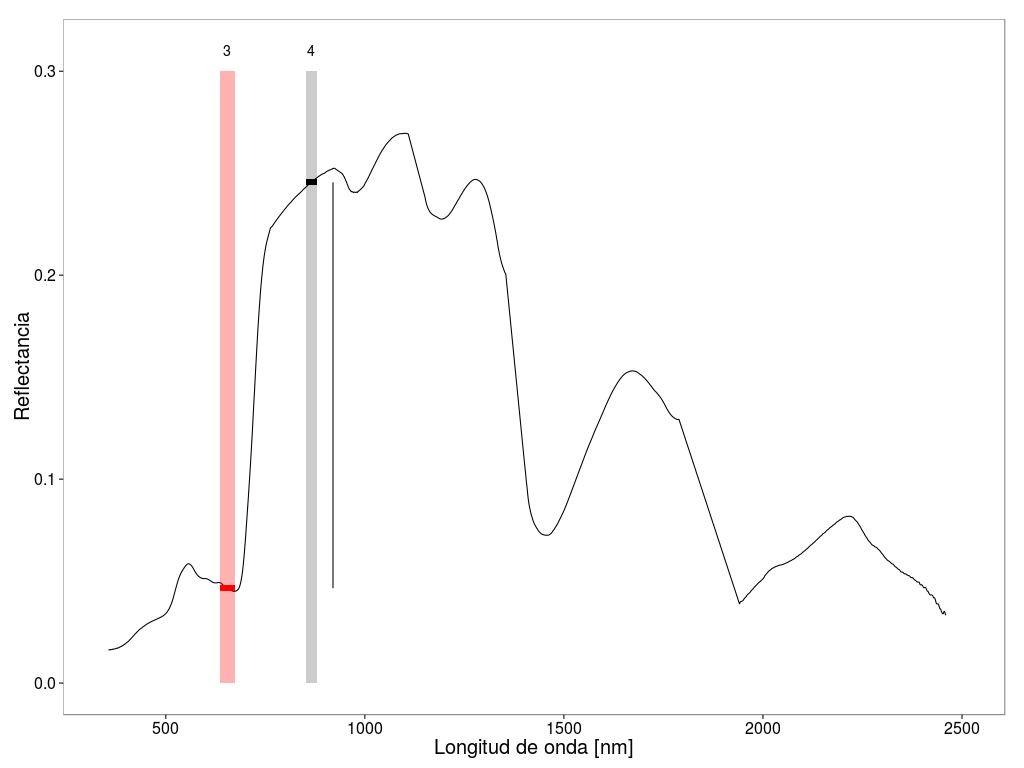
\includegraphics[width=0.8\textwidth]{imagenes/salto_nr.png}
    \caption{Salto de reflectancia entre la regi\'on entre el rojo y el infrarrojo cercano.\footfullcite{clark2007usgs}}
    \end{figure}
\end{frame}
%--- Next Frame ---%
\begin{frame}{\'Indices de Vegetaci\'on}
  \begin{block}{NDVI}
      \begin{equation}
          NDVI = \frac{\rho_n-\rho_r}{\rho_n+\rho_r} 
      \end{equation}
  \end{block}\pause
    \begin{block}{Observaci\'on}
        \begin{itemize}[<+->]
            \item Funciona bien cuando el canopeo es intermedio.
            \item La reflectancia del suelo lo puede afectar.
            \item Satura cuando el canopeo es muy denso.
        \end{itemize}
    \end{block}
\end{frame}
%--- Next Frame ---%

\begin{frame}{\'Indices de Vegetaci\'on}
  \begin{block}{SR}
     $$SR=\frac{\rho_n}{\rho_r}$$
  \end{block}\pause
  \begin{block}{Observaci\'on:}
      \begin{itemize}[<+->]
        \item Satura al igual que el NDVI
        \item Puede mejorar el contraste con vegetaci\'on muy densa
        \item Reduce su efectividad cuando varia la reflectancia del suelo.
    \end{itemize}
  \end{block}
\end{frame}
%--- Next Frame ---%

\begin{frame}{\'Indices de Vegetaci\'on}
  \begin{block}{Observaci\'on}
    Se relaciona con el anterior como $$\frac{\rho_n/\rho_r-1}{\rho_n/\rho_r+1}$$
  \end{block}
\end{frame}
%--- Next Frame ---%

\begin{frame}
    \frametitle{\subsecname}
    \begin{figure}
    \begin{center}
        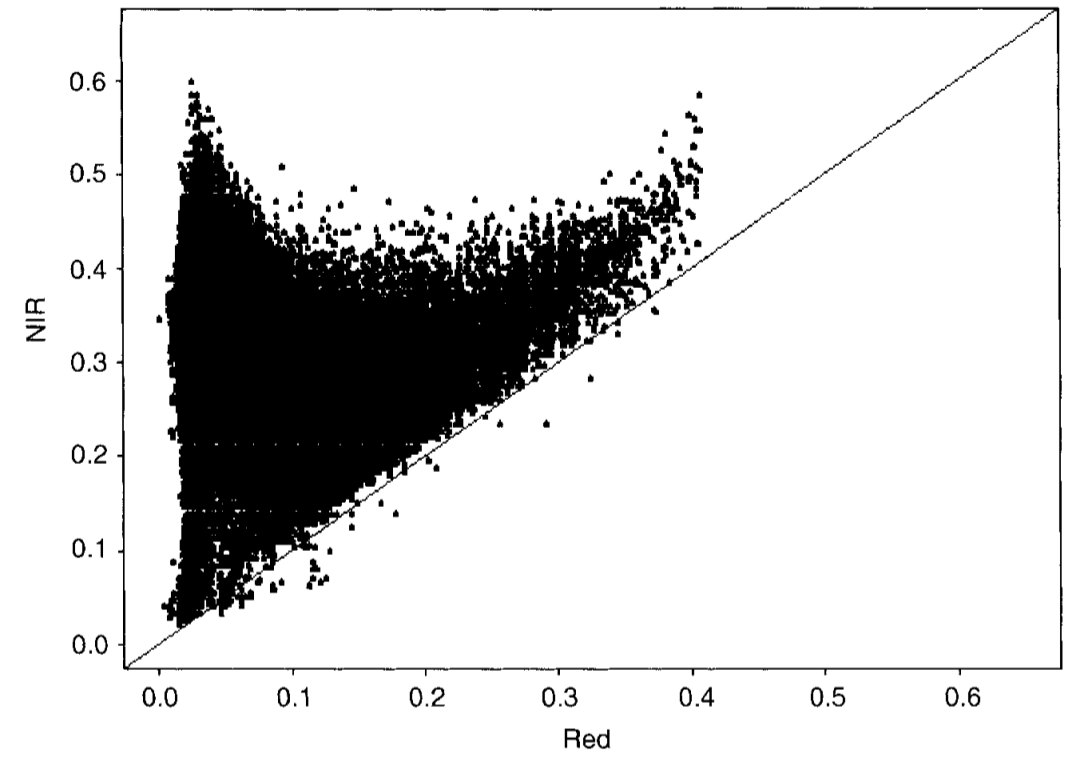
\includegraphics[width=0.8\textwidth]{imagenes/scatter82.png}
    \end{center}
        \caption{Scatterplot nir-rojo en el espacio espectral. \footfullcite{liang2005quantitative}}
    \end{figure}
\end{frame}

\begin{frame}
    \frametitle{\subsecname}
     \begin{block}{Definici\'on}
        Hablaremos de linea de suelo a la linea en un grafico rojo-nir que toca
        por debajo al triangulo de vegetaci\'on. Sobre ella:
         \begin{equation}
             \rho_n = \gamma \times \rho_r +b
         \end{equation}
     \end{block}
\end{frame}

\begin{frame}
    \frametitle{\subsecname}
    \begin{figure}
    \begin{center}
        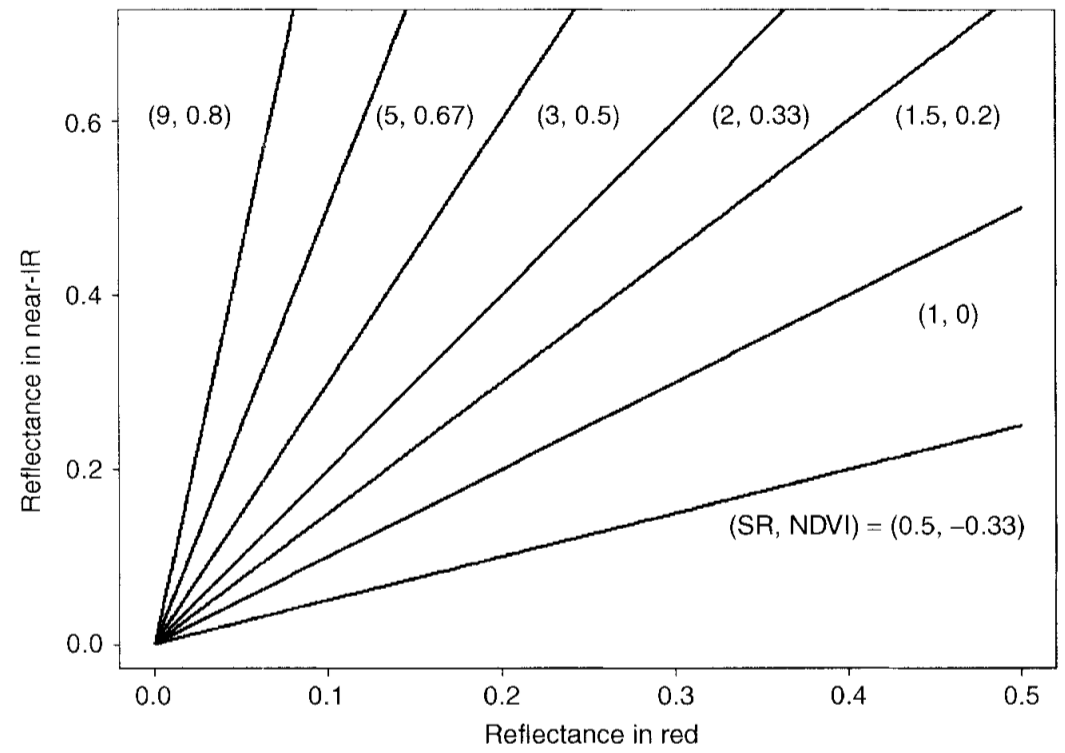
\includegraphics[width=0.8\textwidth]{imagenes/soiline.png}
    \end{center}
        \caption{Distintas pendientes para la linea de
        suelo.\footfullcite{lian2005quantitative}}
    \end{figure}
\end{frame}

\begin{frame}
    \frametitle{\subsecname}
    \begin{block}{Linea de suelo}
        Veamos tres indices que apuntan a eliminar los efectos de la linea del
        suelo sobre el NDVI.
    \end{block}
\end{frame}

\begin{frame}
    \frametitle{\subsecname}
    \begin{block}{SAVI}
        \begin{equation}
            SAVI = \frac{\rho_n-\rho_r}{\rho_n+\rho_r+L}(1+L)
        \end{equation}
    \end{block}\pause
    \begin{block}{Observaci\'on}
        \begin{itemize}[<+->]
            \item Suele ajustar mejor a las variaciones de reflectancia del
                suelo.
            \item Es dif\'icil conocer el valor de $L$ a priori.
        \end{itemize}
    \end{block}
\end{frame}

\begin{frame}
    \frametitle{\secname-\subsecname}
    Existen distintas corrientes sobre como calcular el valor de L
    \begin{equation}
        L=0.5
    \end{equation}\pause
    \begin{equation}
        L = 1-2 a NDVI \times WDVI
    \end{equation}\pause
    donde $a\sim 1.6$
    \begin{equation}
        WDVI = \rho_n -\gamma \rho_r
    \end{equation}
\end{frame}

\begin{frame}
    \frametitle{\secname-\subsecname}
    \begin{block}{TSAVI}
        \begin{equation}
            TSAVI =
            \frac{\gamma(\rho_n-\gamma\rho_r-b)}{\gamma\rho_n+rho_r+\gamma b
            +X(1+\gamma^2)} 
        \end{equation}
        donde $X\sim0.08$.
    \end{block}\pause
    \begin{block}{Observaci\'on}
        \begin{itemize}[<+->]
            \item Compenza algunas variaciones en la reflectancia del suelo.
            \item Compenza variaciones en la densidad del canopeo.
            \item Compenza variaciones por el \'angulo solar.
            \item Compenza variaciones por el cambio en la distribuci\'on
                angular del canopeo.
        \end{itemize}
    \end{block}
\end{frame}

\begin{frame}
    \frametitle{\secname-\subsecname}
    \begin{block}{PVI}
        \begin{equation}
            PVI = \frac{\rho_n-\gamma\rho_r-b}{\sqrt{\gamma^2+1}}
        \end{equation}
    \end{block}\pause
    \begin{block}{Observaci\'on}
        \begin{itemize}
            \item Compenza mejor variaciones en la reflectancia del suelo cuando
                el canopeo es poco denso.
        \end{itemize}
    \end{block}
\end{frame}

\begin{frame}
    \frametitle{\secname-\subsecname}
    \begin{figure}
    \begin{center}
        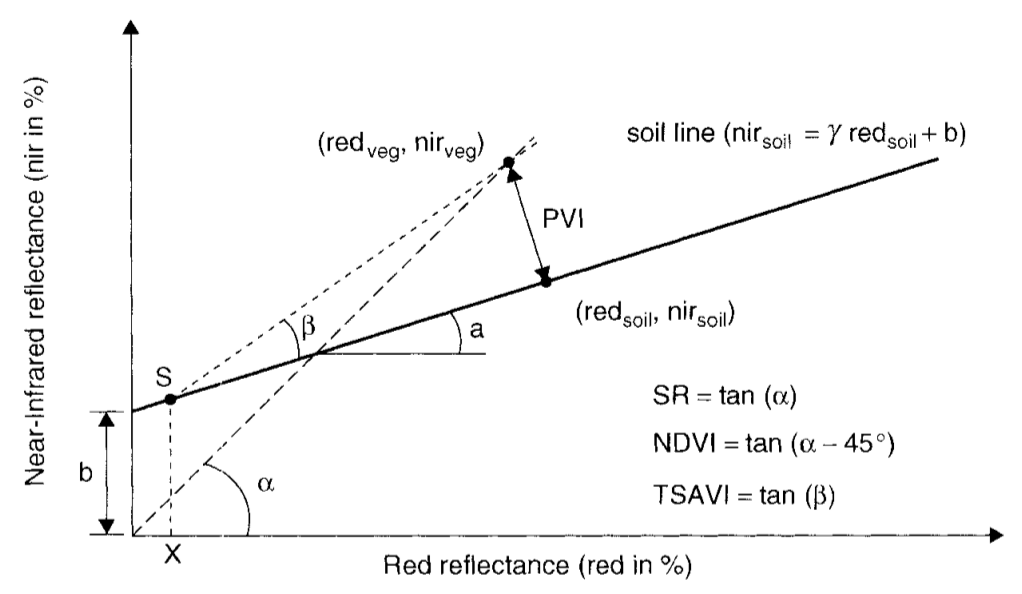
\includegraphics[width=0.8\textwidth]{imagenes/int_graf.png}
    \end{center}
    \caption{Interpretaci\'on de los \'indices en el espacio espectral.\footfullcite{lian2005quantitative}}
    \label{fig:}
    \end{figure}
\end{frame}

\begin{frame}
    \frametitle{\secname-\subsecname}
    \begin{block}{EVI}
        \begin{equation}
            EVI = G\frac{\rho_n - \rho_r}{\rho_n+C_1\rho_r-C_2\rho_b+L}(1+L) 
        \end{equation}
    \end{block}
    donde
    \begin{itemize}
        \item $G  \sim 2.5$
        \item $C1 \sim 6.0$
        \item $C2 \sim 7.5$
        \item $L  \sim 1.0$
    \end{itemize}
\end{frame}

\subsection{Variables biof\'isicas}

\begin{frame}
    \frametitle{\secname-\subsecname}
    En general hablaremos de \'Indices de Vegetaci\'on (VI).\pause
    \begin{block}{Observaci\'on}
        Si tengo una variable $y$\pause
        \begin{equation}
            y = \sum_i a_i VI^i
        \end{equation}
        \begin{equation}
            y = a + b \times VI^c
        \end{equation}
        \begin{equation}
            y = a \log(b-VI)+c
        \end{equation}
    \end{block}
\end{frame}

\begin{frame}
    \frametitle{\secname-\subsecname}
    Estudiemos dos variables biof\'isicas
    \begin{itemize}[<+->]
        \item $F_g$ $\sim$ fracci\'on del suelo cubierto por vegetaci\'on
        \item Biomasa humeda
    \end{itemize}
\end{frame}

\begin{frame}
    \frametitle{\secname-\subsecname}
    \begin{block}{Observaci\'on}
        La relaci\'on entre cada variable biof\'isica y el \'indice debe
        calcularse a partir de mediciones en el terreno.
    \end{block}
\end{frame}

\begin{frame}
    \frametitle{\secname-\subsecname}
    \begin{figure}
    \begin{center}
        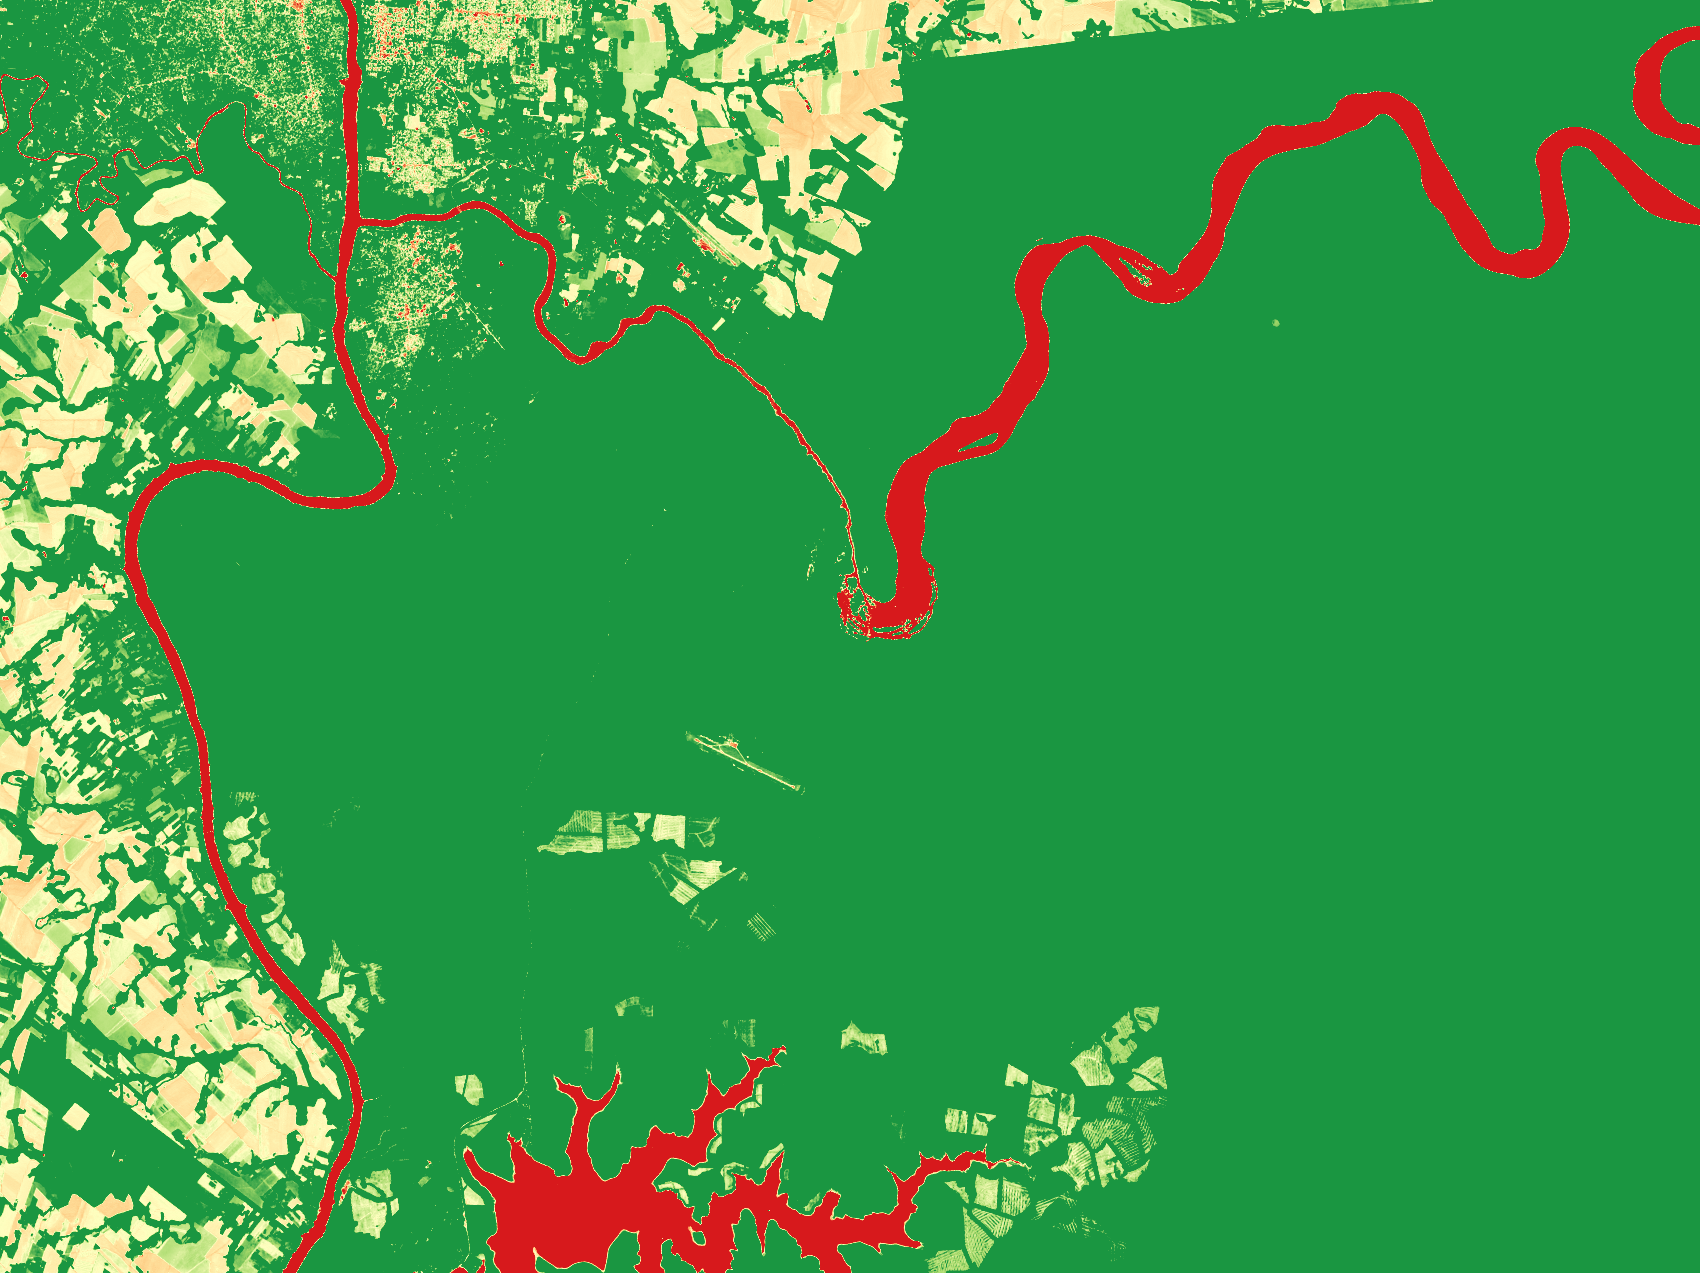
\includegraphics[width=0.8\textwidth]{imagenes/fg.png}
    \end{center}
    \caption{Fracci\'on de suelo cubierta entre 0 y 1 en un mapa de colores.
        Cortes en $0.04$ y $0.52$}
    \label{fig:}
    \end{figure}

\end{frame}

\begin{frame}{\subsecname}
    \begin{figure}
    \centering
    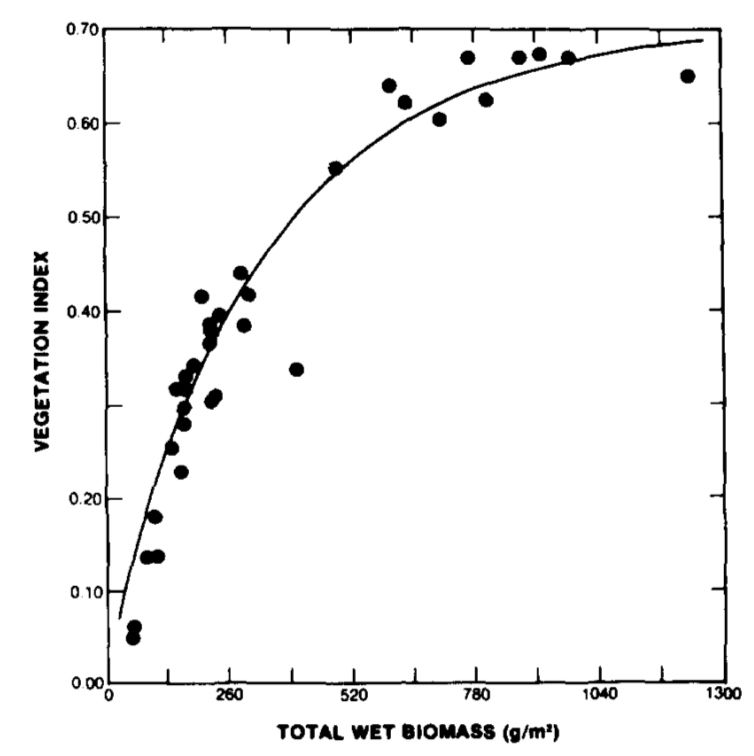
\includegraphics[width=0.6\textwidth]{imagenes/avndvi.png}
    \caption{NDVI vs cantidad de biomasa h\'umeda.\footfullcite{tucker1979red}}
    \end{figure}
\end{frame}
%--- Next Frame ---%



\begin{frame}{\subsecname}
    \begin{figure}
    \centering
    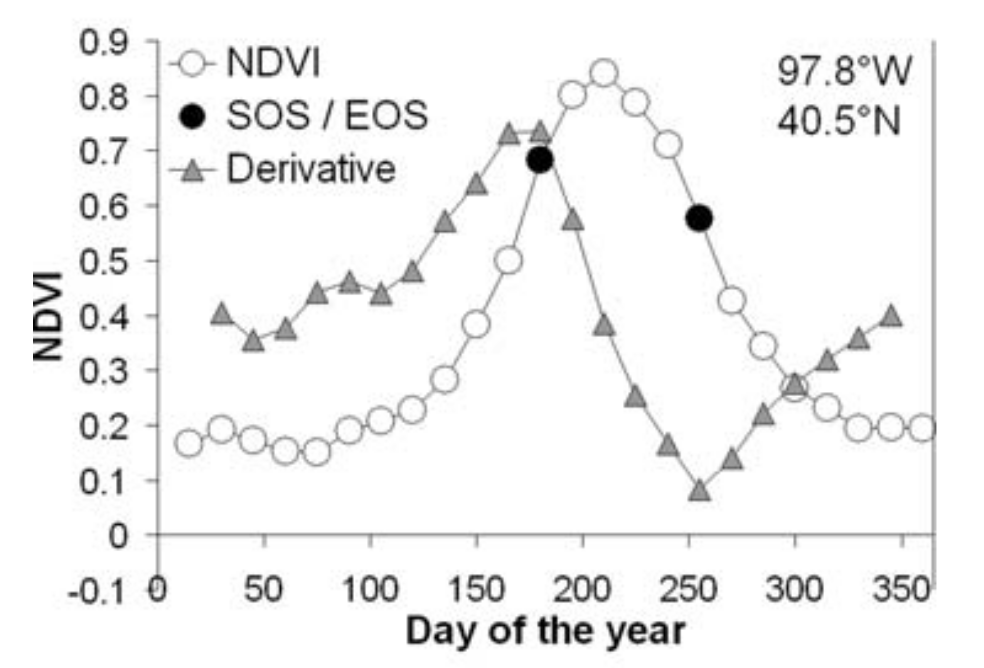
\includegraphics[width=0.8\textwidth]{imagenes/ndvivst.png}
    \caption{Variaci\'on del NDVI en funci\'on de la epoca del año.\footfullcite{de2010spatio}}
    \end{figure}
\end{frame}


\section{Pr\'actica}

\begin{frame}{Pr\'actica}
  \begin{exampleblock}{Actividades pr\'acticas de la tercer clase}
    \begin{enumerate}
      \item Abrir im\'agenes Landsat 8 y digitalizar coberturas de inter\'es.
      \item Calcular el \'indice de vegetaci\'on para las im\'agenes de febrero y agosto.
      \item Realizar curvas fenol\'ogicas a partir del \'indice de vegetaci\'on en la imagen MODIS.
      \item Utilizar la herramienta de componentes principales para reducir la dimensi\'onalidad de la imagen MODIS.
    \end{enumerate}
  \end{exampleblock}
\end{frame}
%--- Next Frame ---%

\end{document}
